\section{Organization plan} %%SW
This part aims to give an overview of the organizational parts of the project, first for the whole project and then for the customer, group and last responsibilities.
\subsection{Organization plan for the whole project}
The distribution of responsibility and an overview of the communication are given in figure\ref{FlowOrg}.
\begin{figure}[h]
	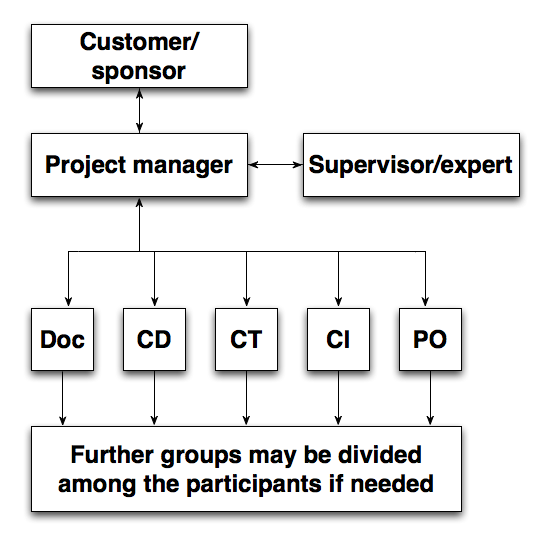
\includegraphics[width=0.7\textwidth]{./Images/FlowChart_Org.png}
	\caption{Overview of responsibility and communication}
	\label{FlowOrg}
\end{figure}
The contact between the customer and the group goes mainly through the project leader. Every group member has his own area of responsibility, and it is then the project manager’s (PM) responsibility to make sure that all the group members work toward the same goal, that no tollgates/milestones are missed, and that there is at least one group member responsible for every task. The PM also divides the project group into smaller groups throughout the project so that the workload is evenly distributed over all the participants. The expert may be consulted when needed to solve parts of the project or when problems occur.
\subsection{The customers organization}
The customer is responsible for approving the tollgates and should be informed/consulted when the milestones are reached.
\subsection{Conditions for the cooperation in the project group}
There is a letter of agreement that will be discussed and developed from the template in Appendix \ref{}. The finished group contract will then be signed by all members.
\subsection{Definition of work contents and responsibilities}
\begin{tabular}{|p{16mm}|p{31mm}|p{100mm}|}
        	\LIPSmilstolpe{\textbf{Name}}{\textbf{Responsibility}}{\textbf{Comment}}
	\LIPSmilstolpe{Simon Wallin}{Project Manager}{Responsible for the general process of the project and that the TG/MS as well as requirements are met. Also to keep track of time logging and contact with the customer.}
	\LIPSmilstolpe{Björn Lindström}{Documents (Doc)}{Responsible for a uniformed documentation and keeping track of meeting protocols.}
	\LIPSmilstolpe{Francois Vrel}{Code Design (CD)}{Has the main responsibility for the design of the code.}
	\LIPSmilstolpe{Simon Larsson}{Code Test (CT)}{Responsible for putting together a test plan and making sure that this is used throughout the project.}
	\LIPSmilstolpe{Johan Jönsson}{Code Implementation (CI)}{Has the main responsibility for making sure that all the code is implemented and also in the best possible manner.a}
	\LIPSmilstolpe{Mohammed Rashed}{Program Operation (PO)}{Has the main responsibility to make sure that the program operates as intended.}
\hline
\end{tabular}